\dev{Emile Martinez}{}

\textit{A compléter}

\begin{com}
	Ici, suivant le temps, à voir si on met un rappel de à quoi sert la pile et à quoi sert le tas.
	Plutot non et faire un schéma qui explique ce que fait le code assembleur à la fin.
\end{com}


\paragraph{But} Stocker ce qui est local (donc pas les malloc).

\paragraph{Idée} Avoir une pile.\\
Si $f$ appelle $g$ qui appelle $h$ $\to$ \raisebox{-.5\height}{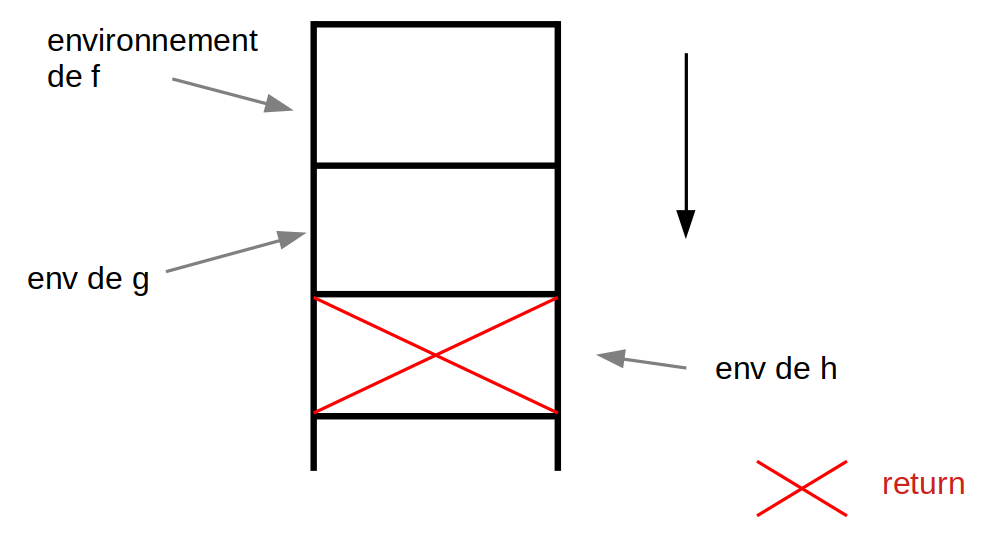
\includegraphics[scale = 0.2]{Developpements/pile d'appel/idee_pile.png}}
\begin{minipage}{0.3\linewidth}
	(ici environnement c'est les variables locales)
\end{minipage}

\paragraph{Lors d'un appel de fonction :}
\begin{itemize}[label=$\star$]
	\item On empile la valeur des arguments de la fonction
	\item On décale le début de la pile\\
	$\rightarrow$ Car on veut que l'appel à une fonction ne dépendent pas du niveau d'imbrication des appels
	\item On alloue sur le sommet de la pile de l'espace pour les variables définies localement.
\end{itemize}

\begin{com}
	Là, on peut commencer l'exemple et revenir écrire le retour de fonction après.
\end{com}

\paragraph{Lors d'un return :}
\begin{itemize}[label=$\star$]
	\item Calculer la valeur de retour
	\item Enlever de la pile toutes nos variables
	\item Remettre la pile à son début précédent
	\item Ecrire sur le sommet la valeur de retour
	\item Le code appelant lis la valeur sur le sommet
\end{itemize}

\paragraph{Exemple d'exécution de code} \enspace \\

\begin{minipage}{0.25\linewidth}
\begin{lstlisting}
<@\color{red} int f(int x)\{@>
    <@\color{red} int y;@>
    <@\color{red} y = x+1;@>
    <@\color{red} x = x*y;@>
    <@\color{red} return x;@>
<@\color{red}\}@>

<@\color{green} int g(int x, int y)\{@>
    <@\color{green} int z;@>
    <@\color{green} z = 0;@>
    <@\color{green} z = f(x);@>
    <@\color{green} z = z + f(y);@>
    <@\color{green} return z;@>
<@\color{green}\}@>

<@\color{blue} int main()\{@>
    <@\color{blue} int x,y;@>
    <@\color{blue} x = 1;@>
    <@\color{blue} y = 2;@>
    <@\color{blue} x = g(x+2, y);@>
<@\color{blue}\}@>
\end{lstlisting}
\end{minipage}\quad \begin{minipage}{0.70\linewidth}
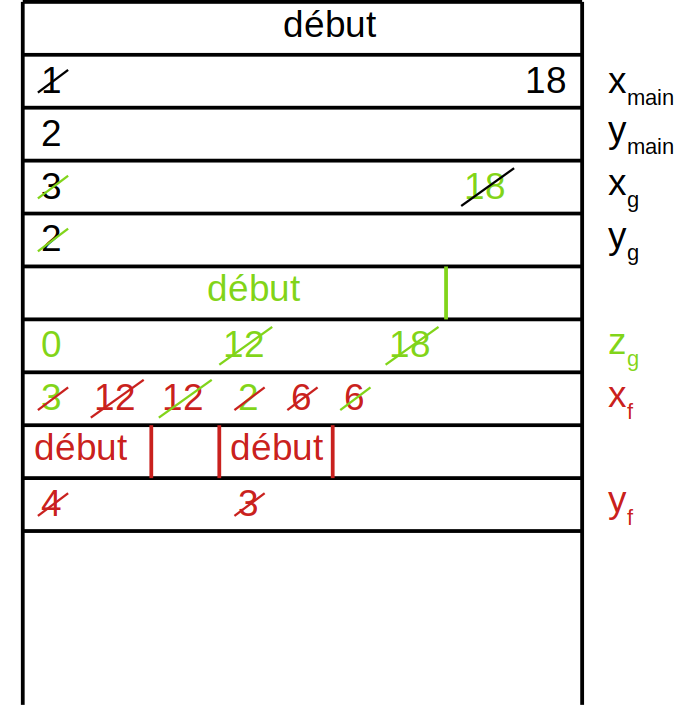
\includegraphics[scale=0.4]{Developpements/pile d'appel/exemple_pile.png}
\end{minipage}

\paragraph{Comment faire ça en assembleur ?}

On se réserve deux registres, que le code ne touchera pas : $b_p$ (pour base pointer, la base de la pile) et $s_p$ (pour stack pointer, le sommet de la pile).

\paragraph{Idée} $b_p$ pointe vers «début» et «début» stocke le $b_p$ précédent. $s_p$ pointe vers le sommet de la pile.

\begin{minipage}{0.3\linewidth}
\begin{lstlisting}
y = f(x1, ..., xn)
\end{lstlisting}
\end{minipage} \qquad $\longrightarrow$ \qquad
\begin{minipage}{0.5\linewidth}
	\begin{lstlisting}
// mettre dans r1 la valeur de x1
store r1 [sp]
iadd sp sp 1
...
// mettre dans r1 la valeur de xn
store r1 [sp]
iadd sp sp 1

call f // va au code de f
//mettre dans r1 l'adresse de y
iadd sp sp -1
load r2 [sp]
store r2 [r1]
	\end{lstlisting}
\end{minipage}

\enspace\\
\begin{minipage}{0.3\linewidth}
	\begin{lstlisting}
int f(x1, ..., xn){
    int y1, ..., ym;
    //code de f
    return yi;
}
\end{lstlisting}
\end{minipage} \qquad $\longrightarrow$ \qquad \begin{minipage}{0.5\linewidth}
\begin{lstlisting}
store bp [sp]
mv sp bp
iadd sp sp 1

iadd sp sp m;

// code de f

iadd r1 bp (i+1)
load r2 [r1]
iadd sp bp -n
load bp [bp]
store r2 [sp]
ret //revient au code appelant
\end{lstlisting}
\end{minipage}